\documentclass{beamer}
\usepackage{mathtools, amsmath, xcolor, graphicx}
\usetheme{Rochester}
\usecolortheme{dolphin}

\author{Joe Bentley and Jake Lane}

\title{Higgs Signal Optimisation}

\institute{}
\subject{Physics}
\date{}
\begin{document}


\frame{\titlepage}


\frame{
\frametitle{Summary}
\begin{enumerate}
\item General background on Higgs
\item How Higgs signals are simulated
\item How the signals are interpreted
\item How the Higgs signal is optimised
\item Problems in optimisation and improvements
\item Possible expansions of the project
\end{enumerate}
}


\frame{
\frametitle{Background}
The Higgs boson is produced in many channels.
\pause
The most common in proton collider experiments is 'gluon gluon Fusion' (ggF)
\begin{figure}
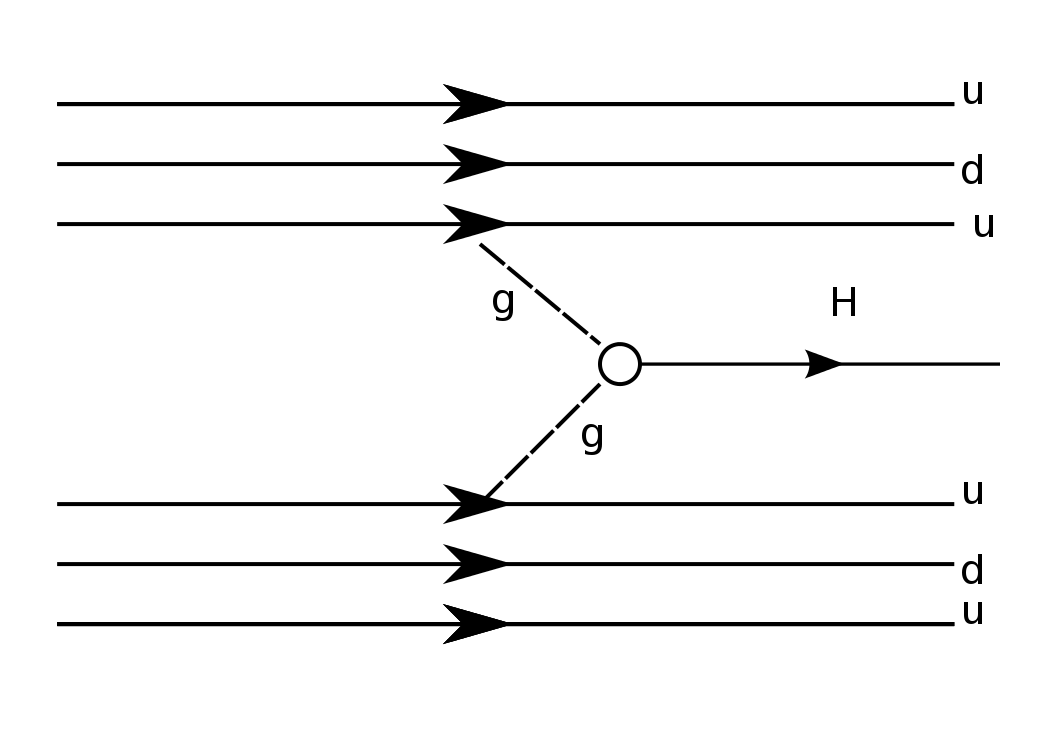
\includegraphics[scale = 0.1]{VBF.png}
\caption{Gluons fusing into a Higgs at a proton-proton interaction}
\end{figure}
\pause
The Higgs decays in a very short period of time in many channels, the most common is 2 bottom quarks, but we investigate the decay into 2 photons (the diphoton channel.)
}

\frame{
\begin{figure}
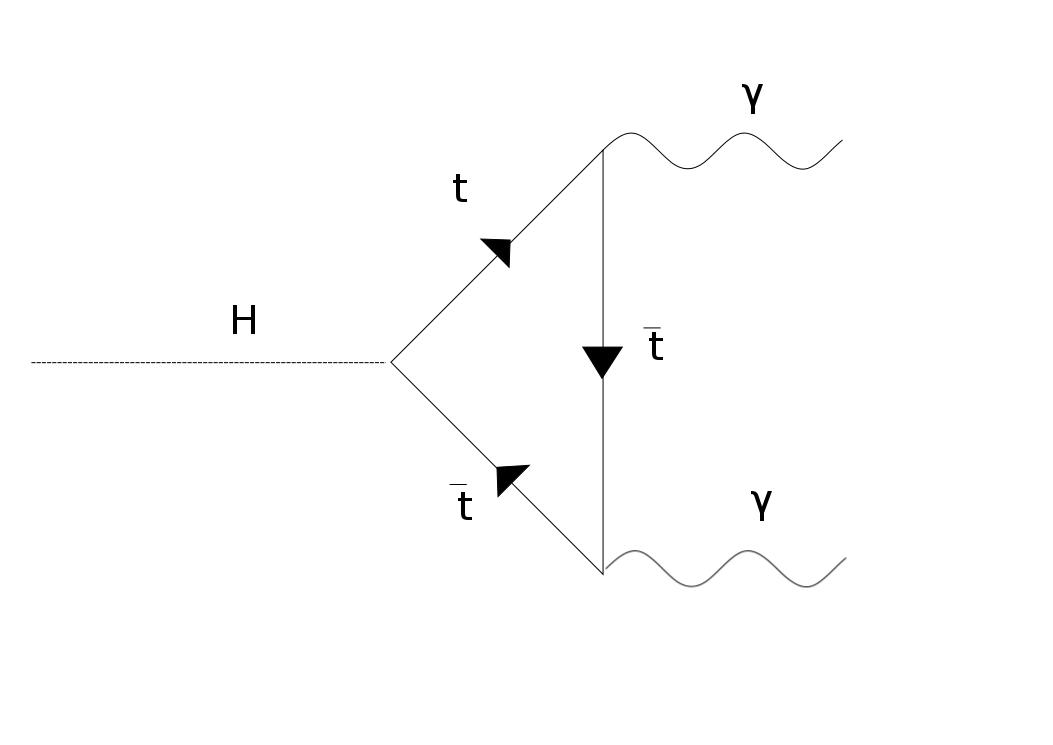
\includegraphics[scale=0.2]{Hyy.png}
\caption{Decay of Higgs into 2 photons}
\end{figure}
This has a branching fraction of order of $10^{-3}$ but is much easier to detect experimentally.
}


\frame{
\frametitle{Simulation}

The Higgs events and background events are simulated using PYTHIA. The simulation consists of a text file of the Energy and momentum (4 momentum) of each photon in each event (read collision.) We will use 1 simulation of Higgs events (which still have background in them) and 1 simulation of background events.
}

\frame{
\frametitle{Parsing}

\begin{itemize}
  \item We use a script written in Python 3 to parse the event data from the four momenta
  \item It calculates the invariant mass of each decay event and outputs this to a plaintext file for plotting
  \item It can also apply a range of filtering on the events to filter out events that are not Higgs
  \item The script is written as a library so that we can use its features from other scripts, like our filter optimisation scripts
\end{itemize}
}

\frame{
  \frametitle{Terms}

  Transverse momentum is the component of momentum perpendicular to the beam axis.

  etc.. (explain so the audience aren't too confused about particle physics terms)
}

\frame{
\frametitle{Weighting}

In our simulated data, there are 10,000 Higgs events, and 1,000,000 background events. In an actual collider experiment this ratio would be much lower. To account for this we need to apply weightings to each dataset.

\pause

\begin{align*}
  \frac{\text{num. Higgs events}}{\text{num. background events}} = \frac{\sigma{\left(\text{Higgs produced}\right)} \times B_f\left(H\to\gamma\gamma\right)}{\sigma{\left(\text{background}\right)}}
\end{align*}

By knowing the branching factor of the Higgs to two photons decay, as well as the cross sections of the background and of the Higgs production, we can use the above equation to calculate how much weighting we need to apply to the Higgs or background events in our histogram.
}


\frame{
\frametitle{Filtering}

\begin{itemize}
  \item There are $\sim$ 100 Higgs events to $\sim$ 100,000,000 background events
  \item If we do not have good filtering then there is no chance of seeing the Higgs events amongst the background events
  \item We need an effective way to distinguish Higgs events from background events
\end{itemize}
}

\frame{
  \frametitle{Filter Methods}

  \begin{enumerate}
    \item Transverse momentum filtering
    \item Pseudorapidity filtering
    \item Azimuthal angle filtering
  \end{enumerate}
}

\frame{
\frametitle{Optimising our Filters}

To optimise our filters so that we have the best ratio of Higgs events to background events, we need to optimise our filter methods for the highest statistical significance $\Sigma$,

\begin{equation}
\Sigma \equiv \frac{S}{\sqrt{S + B}}
\end{equation}

where $S$ is the number of filtered signal events and $B$ is the number of filtered background events.

\pause

We apply the filtering and calculate the significance for a series of different parameters, for example for different transverse momenta cuts, to see what gives us the best statistical significance.
}

\frame{
\begin{figure}
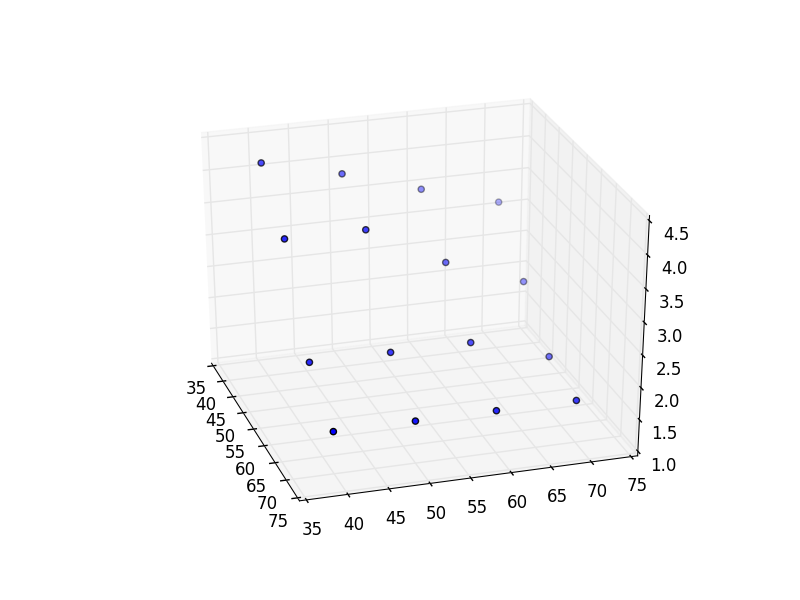
\includegraphics[scale=0.2]{significance1}
\caption{Statistical significance (height of points) for a series of different transverse momenta}
\end{figure}

This is a 3D plot generated from a script that calculates the statistical signifiance for various transverse momenta cuts. From graphs like these we can narrow down the ranges of transverse momenta that we filter until we get the highest statistical significance. We use PyPlot to generate our plots.
}

\frame{
\frametitle{Seeing the Higgs}

Actually observing it explanation
}

\frame{
\frametitle{Issues}
}

\frame{
\frametitle{Further Explorations}
}

\frame{
\frametitle{Conclusion/Questions}
}

\end{document}
